


%%%%%%%%%%%%%%%%%%%%%%%%%%%%%%%%%%%%%%%%%%%%%%%%%%%%%%%%%%%%%%%%%%%%%%%%%%%%%%%%%%%%%%%%%%%%%
%%									Chapitre 3												%
%%%%%%%%%%%%%%%%%%%%%%%%%%%%%%%%%%%%%%%%%%%%%%%%%%%%%%%%%%%%%%%%%%%%%%%%%%%%%%%%%%%%%%%%%%%%%


{\chapter[Deploying nematode-resistant plants ]{Un modèle démo-génétique d'interaction entre plantes et nématodes pour un déploiement optimal des gènes de résistance} \label{article}
\label{chapter_3}}
	\minitoc
	\newpage

%%%%%%%%%%%%%%%%%%%%%%%%%%%%%%%%%%%%%%%%%%%%%%%%%%%%%%%%%%%%%%%%%%%%%%%%%%%%%%%%%%%%%%%%%%%%%

\iffalse
Les nématodes à galles (RKNs) sont des ravageurs du sol qui ont un impact économique majeur dans le monde entier. Ils sont considérés comme l'un des pathogènes les plus importants au monde \citep{Trudgill2001}. Dans les plantes, des gènes de résistance dits majeurs, fonctionnant selon le modèle « gène pour gène », ont été identifiés.  L'utilisation au champ de plantes résistantes est perçu comme un des moyens les plus efficaces pour contrôler les nématodes \citep{Roberts1990}. 
Les résistances peuvent être utilisées de plusieurs manières dans le cadre de la lutte contre les nématodes en cultures maraîchères : (i) classiquement, en cultivant une variété agronomique porteuse d'un seul gène de résistance (ii) en rotations des cultures  entre les cultures  agronomiques  plus sensibles ou des cultures non-hôte    
 \citep{Djian-Caporalino2014}. L'utilisation de résistances en rotation peut s'intégrer aussi dans des prototypes de système de culture qui combinent   d'autres pratiques agronomiques à l'interculture : plante pièges, plantes biofumigantes et  solarisation.
\fi

\thispagestyle{empty}
L’utilisation de variétés  résistantes
est une voie en plein essor qui se heurte à des défis majeurs. Premièrement,
le nombre  d’espèces végétales avec des variétés commercialisées porteuses de gènes de résistance aux nématodes est limité (seulement tomate et piment en maraîchage). De surcroît, l'apparition de génotypes virulents, à même de contourner les résistances,  remet potentiellement en cause la durabilité de ces méthodes de lutte, à l'échelle de la parcelle comme de l'exploitation \citep{Jarquin-Barberena1991,Djian-Caporalino2011,Djian-Caporalino2014}. Fort heureusement, la virulence chez les nématodes est généralement associée à un coût de fitness sur les plantes sensibles et résistantes, représenté par une diminution de la fertilité et de la fécondité \citep{Castagnone-Sereno2007,Djian-Caporalino2011}. Ainsi, si les nématodes virulents sont sélectionnés en cas d'usage de plantes résistantes, ils sont aussi contre-sélectionnés en cas d'usage de plantes sensibles au profit de nématodes avirulents.
De plus, puisque les nématodes ont une faible capacité de dispersion intrinsèque, l'alternance entre les  plantes résistantes et sensibles en rotation serait  une stratégie plus appropriée qu'une stratégie basée sur l’arrangement spatial des hôtes.

 Nous  proposons  un modèle décrivant la dynamique saisonnière d'une population de nématodes à galles à l'échelle d'une plante grâce à un formalisme semi-discret \citep{Mailleret2009}. Le modèle sur lequel nous avons travaillé décrit la dynamique de croissance d’une plante infectée par des nématodes au cours des saisons de culture, 
  alternant avec un épisode discret de survie du nématode dans le sol entre les saisons.
À partir de ce modèle, le but de notre travail a été de rechercher  des stratégies optimales de rotation de plantes résistantes et  sensibles afin de maximiser le rendement moyen saisonnier.
 L'optimisation a été réalisée  pour différents scénarios épidémiologiques en interaction avec différents gènes majeurs de résistances.  Nous avons également testé la robustesse de nos résultats pour
déterminer si l'efficacité des rotations périodiques optimales peut
être maintenue suite à des variations dans les valeurs de paramètres du modèle. 
La rotation des cultures s'est avérée être une stratégie de lutte efficace. Elles se caractérise par de faibles ratios de plantes résistantes.

 Nous proposons  dans la suite notre article publié le 04 Mai 2020 dans le journal  \textit{Evolutionary Applications} (volume 13, pages 2206-2221). Cet article de journal fait office de \autoref{article} du manuscrit de thèse.



\selectlanguage{english}
%\bibliographystyle{newphy}
%\bibliography{mybiblio}

\newpage
% Début du chapitre

%\section{Le modèle simple d'étude }
%\subsection{Description du modèle}
%\subsection{$R_0$ inter-saison}  
%\subsection{$R_0$ intra-saison} 

%\section{Article}

\title{Multiseasonal modelling of plant-nematode interactions reveals efficient plant resistance deployment strategies}

\author{Samuel Nilusmas$^{1,2}$, Mathilde Mercat$^1$, Thomas
Perrot$^1$, Caroline Djian Caporalino$^1$, 
Philippe Castagnone-Sereno$^1$, Suzanne Touzeau$^{1,2,*}$, Vincent
Calcagno$^{1,*}$,  and Ludovic Mailleret$^{1,2,*}$}

\date{$^1$Université Côte d'Azur, INRAE, CNRS, ISA, Sophia Antipolis, France;
  $^2$Université Côte d'Azur, Inria, INRAE, CNRS, Sorbonne Université,
  BIOCORE, Sophia Antipolis, France\\[1ex]
  Author for correspondence: \\
  Samuel Nilusmas: samuel.nilusmas@gmail.com\\[1ex]
  $^*$These authors should be considered joint senior author.
}
\maketitle




\bigskip
\par\noindent


\bigskip
\par\noindent{Funding Information}\\
INRAE, France\\
Région Sud PACA, France 

% ***************   ABSTRACT    ***************%
{
\bigskip
\noindent\rule{\linewidth}{.2mm} \\[5mm]
\selectlanguage{english}
\textsc{summary}
\medskip

\begin{itemize}
\item Root-knot nematodes, \textit{Meloidogyne spp.}, are soil-borne
  polyphagous pests with major impact on crop yield
  worlwide. Resistant crops efficiently control avirulent root-knot
  nematodes, but favour the emergence of virulent
  forms. Since virulence is associated with fitness costs,
  susceptible crops counter-select virulent root-knot nematods.  In
  this study we identify optimal rotation strategies between
  susceptible and resistant crops to control root-knot nematodes and
  maximize crop yield.
\item We developed an epidemiological model describing the
  within-season dynamics of avirulent and virulent root-knot nematodes
  on susceptible or resistant plant root-systems, and their
  between-season survival. The model was fitted to experimental data
  and used to predict yield-maximizing rotation strategies, with
  special attention to the impact of epidemic severity and genetic
  parameters.
\item Crop rotations were found to be efficient under realistic
  parameter ranges. They were characterised by low ratios of resistant
  plants, and were robust to parameter uncertainty. Rotations provide
  significant gain over resistant-only strategies, especially under
  intermediate fitness costs and severe epidemic contexts. Switching
  from the current general deployment of resistant crops to custom
  rotation strategies could not only maintain or increase crop yield,
  but also preserve the few and valuable R-genes available.
\end{itemize}

\par\noindent\textbf{Keywords:} computer simulation, crop protection, disease resistance, mathematical model, nematode infections, pest control, population dynamics, rotation, seasons, virulence




%******************   SECTION INTRODUCTION   ***************%

\section{Introduction}

As the global population increases, finding effective and durable
crop protection strategies has become a major challenge \citep{Cunniffe2015}.
Predictions indicate that population growth, combined with changes in
dietary habits, will lead to an increase in the global food demand
by at least $50\%$ in 2050 \citep{Tilman2011,Springmann2016}. To meet
this demand, crop production will have to increase, with expected
negative environmental impacts (biodiversity and forest loss, reduced
freshwater availability, soil degradation and CO2 emissions) if relying
on the extensive use of chemical pesticides and monocultures \citep{Tilman2001,Stoate2009,Zhan2015}.
Furthermore, crop losses are expected to increase as well, owing to
the emergence or evolution of plant pests and diseases \citep{Palumbi2001,Stukenbrock2008}.
These trends call for experimental and theoretical studies aiming at
protecting crops and increasing their yield durably, while reducing
pesticide dependence. In this context, the development of
environmentally-friendly pest management strategies based on
biological control, better cultural practices and the use of resistant
plants are very promising \citep{Mundt2014,Zhan2015,vanLenteren2018}.

Natural plant resistance is among the most efficient alternatives
to pesticides in economic, environmental and social terms.
Qualitative plant resistance rests on gene-for-gene interactions \citep{Flor1971},
in which an avirulent gene (Avr-gene) in the pest or pathogen interacts
with a major resistance gene (R-gene) in the plant, resulting in disease
resistance through what is usually called effector-triggered immunity
or incompatible reaction \citep{Dangl2001,Jones2006}. If the R-gene
is inactive or absent, or equivalently if the pest lacks the Avr-locus,
the interaction instead results in plant infection. Major R-genes
are rare in nature and plant breeders mostly work on the introgression
of a small list of major R-genes into different genetic backgrounds
to create commercial crop cultivars. Therefore, farmers ultimately
employ the same resistance genes over several years and on large spatial
scales. Such an intensive use of resistance generates strong selection
pressures on populations of avirulent pests, that can lose the Avr-gene
through mutation, causing the emergence and establishment of virulent
variants \citep{Leonard1977,Castagnone-Sereno2002,McDonald2002,Parlevliet2002,Garcia-Arenal2003}.

According to \citet{Johnson1981}, a durable resistance is one that
remains effective in a cultivar for a long period of time despite its
widespread cultivation. In a gene-for-gene system,
resistance durability may depend on the time required for a mutation
at the Avr-gene to occur and the time for the virulent pathogen to
establish
\citep{vandenBosch2003,Stuthman2007,Barrett2008,Fabre2009,Brown2015,Zhan2015}.
The latter might be expected to be very short, considering the huge
advantage for a pathogen to overcome resistance and become virulent.
However, significant polymorphism exists at virulence genes, that can
at least partly be explained by fitness costs associated with
virulence \citep{Stahl1999,Tian2003,Laine2008}. Numerous studies have
reported fitness costs in bacteria \citep{Cruz2000,Leach2001},
oomycetes \citep{Montarry2010} or viruses \citep{Garcia-Arenal2013}.
The existence of fitness costs implies that even though virulent
pathogens are selected for in resistant crops, they are selected
against in susceptible crops, where avirulent pathogens grow and
reproduce faster.

Several approaches to improve the durability of resistant
  genes have been proposed
  \citep{vandenBosch2003,Fabre2012,Papaix2014,Fabre2015,Lof2017}.  The
  most common deployment strategies are mixtures, mosaics and
  rotations of resistant and susceptible plant cultivars, all of
  which exploit spatial and/or temporal heterogeneity in selection
pressures
\citep{Kiyosawa1982,Mundt2002,Pink2002,Djidjou-Demasse2017,Rimbaud2018}.

Root-knot nematodes (\textit{Meloidogyne spp.}, Kofold \& White) are
ubiquitous plant pathogens \citep{Trudgill2001,Jones2011}. They are
obligate extremely polyphagous plant endoparasites, that cause
damage to the roots of thousands of host plant species
\citep{Perry2009, Wesemael2011}.  Overall, their economic impact has
been estimated at over 121 billion dollars of crop losses each year
\citep{Chitwood2003}.  For several decades, controlling these
parasites has relied on chemical treatments, but these proved
extremely damaging to the environment and to human health and have
been banned \citep{Zasada2010,Abad2010}. {Root-knot nematode
  infestations are becoming an increasing source of concern in
  vegetable production due to these recent restrictions on the use of
  chemical nematicides. For instance, a survey by
  \citet{Djian-Caporalino2012} showed that in the South of France,
  more than $40\%$ of horticultural holdings are impacted by root-knot
  nematodes, sometimes with insurmountable financial consequences.
The fight against root-knot nematodes {is now therefore
  largely based on the use of plant cultivars bearing resistance
genes \citep{Williamson2009}. However, resistance breaking by virulent
nematodes has been demonstrated in the laboratory
\citep{Jarquin-Barberena1991,Djian-Caporalino2011,Meher2009} and
{is more and more observed in field conditions
  \citep{Verdejo-Lucas2009}.

As for other plant parasites, virulence in root-knot
  nematodes is associated with a fitness cost and it was shown that
virulence reduces the capacity to infect the plant, as well as the
number of eggs laid per female
\citep{Castagnone-Sereno2007,Djian-Caporalino2011}.  Therefore,
setting up rotation strategies of resistant and susceptible cultivars
has the potential to increase the durability of resistance genes and
the efficacy of resistance–based nematode control.  However, field
tests of deployment strategies in terms of epidemic control and
resistance durability remain difficult, owing to their labor intensive
nature and to the long time horizons involved
\citep{Djian-Caporalino2014}.

In these conditions, modelling approaches constitute a powerful way to
explore resistant plant deployment strategies and assess their
efficiency to reduce yield losses and increase control durability
\citep{Brown2015,Papaix2018}. {The} literature is very poor in
theoretical modelling studies addressing the control of soil-borne
pathogens with limited dispersal, such as {root-knot nematodes}. For
instance, most studies deal with pathogens that can disperse over
large spatial scales
\citep{Gilligan1995,Thrall1997,Otten2006,Fabre2012,Djidjou-Demasse2017,Lof2017}. {Root-knot
  nematodes}, in contrast, have very limited mobility in the soil,
feeding and reproducing locally in the plant root
system. Consequently, nematode populations barely mix and strategies
based on spatial arrangements are poorly applicable. In addition, the
major {root-knot nematode} species reproduce solely by clonal
reproduction so that techniques based on recombination between
virulent and avirulent genotypes do not operate.

The purpose of this study was to assess quantitatively whether
rotation strategies between susceptible and nematote-resistant
cultivars can efficiently control nematodes, and to
determine which optimal crop rotation strategies should be used to
maximize crop yield over several seasons. We did this by building a
semi-discrete plant epidemic model \citep{Fabre2012, Mailleret2009,
  Mailleret2012}, tailored to the {root-knot nematode}
pathosystem. The model describes the within-season dynamics of the
interaction between a plant root system and {root-knot nematodes}, the
owerwintering dynamics between consecutive seasons and the potential
evolution of the nematode population from avirulent to virulent
forms. The model was parameterized from the literature and fitted to
experimental data \citep{Ehwaeti1998}.  We used the model to compute
optimal crop rotation strategies with respect to a proxy of crop yield
over different time horizons. Given that the fitness costs vary among
R-genes and nematode strains, and are crucial to the durability of
R-genes, we payed special attention to the influence of these genetic
parameters. We evaluated to what extent crop rotation provided better
crop yield than the widely used resistant plant-only strategy (pure
resistant strategy) for different epidemic scenarios and genetic
parameters. We also tested the robustness of our results to determine
whether the effectiveness of optimal periodic rotations can be
maintained even if epidemiological and genetic parameters are not
known precisely. We investigated the key factors to be taken into
account for optimal resistance plant deployment strategies against
{root-knot nematodes}.


% ******************   SECTION MATERIAL & METHODS   ***************%

\section{Materials and methods}

We developed and applied a model of the interaction between crop
plants and a nematode pest. Plants can be either resistant or
susceptible, and the nematodes can be either virulent or
avirulent. Resistant plants do not get infected by the avirulent
nematodes but they do prompt the evolution of virulent
nematodes. Thus, there is a potential trade-off. In the short term,
resistant plants give higher yields because they are not infected by
the nematodes. However, in the longer term, strategies that include
susceptible plants can give higher yields by keeping the levels of
virulence in the nematodes lower. We used the model, parameterised to
a real world system of economic importance, to investigate the
trade-offs between these strategies. Furthermore, we studied the
influence of parameter values, by implementing contrasted epidemic
scenarios and performing a robustness analysis.

\subsection{Study system}

We focused on root-knot nematodes of the species \textit{Meloidogyne
  incognita} (Kofold \& White). These are obligate endoparasites of
plant roots, and reproduce only by clonal reproduction. \textit{M.\
  incognita} is one of the most prevalent species in the warm
conditions of Mediterranean countries, especially in protected crops
\citep{Wesemael2011}. It is one of the most serious concerns for
tomato growers in the South of France and other Mediterranean
countries, for instance in Morocco where tomatoes are still
planted for many consecutive years.

The life cycle of \textit{M.\ incognita} consists in four stages that
can be achieved in three to five weeks, depending on environmental
conditions \citep{Abad2010}. Second-stage juveniles dwell in the soil
and penetrate the plant when a root grows in their vicinity. Once a
nematode reaches the vascular cylinder of the root, salivary
secretions induce the creation of a feeding site. These are composed
of five to six hypertrophied plant cells, known as giant cells. The
nematode spends the rest of its life in this feeding site, where it
develops until reproduction.  When mature, adult females release
several hundreds of eggs (between $300$ to $2000$ eggs/female on 
average) outside the root, that will hatch into
free living juveniles and complete the cycle
(\autoref{fig1}a).

\begin{figure}[ht]
  \centering 
   \includegraphics[width=\linewidth]{fig1.pdf} 
  \caption[(a) Life cycle of root-knot nematodes
     and (b) Schematic description of model
      \eqref{sys0}.]{\textbf{(a)} Life cycle of root-knot nematodes
      (adapted from \citet{Williamson2003} and
      \citet{Abad2010}). \textbf{(b)} Schematic description of model
      \eqref{sys0}. Root-knot nematode eggs hatch as J2 larvae (free
      living nematodes $P$) which can penetrate healthy parts of plant
      roots (healthy roots $H$). After infection, the larva migrates
      down to the root tip, enters the vascular cylinder and migrates
      up the root to settle and induce a feeding site on host cells
      (giant cells, latently infected roots $E$). The nematode ingests
      the cytoplasm of the giant cells to maturate into a pear-shaped
      mature female that releases its eggs onto the root surface
      (infectious roots $I$) in a protective matrix (egg mass). When
      conditions are favourable, eggs hatch and the cycle starts
      again. Text colors match between both panels.}
  \label{fig1} 
\end{figure}

In the \textit{Solanaceae} plant family, a few resistance genes are
known to block the development and reproduction of root-knot
nematodes: the \textit{Mi-1} gene in tomato (Lycopersicon
lycopersicum, Linnaeus) \citep{Milligan1998} and the\textit{ N},
\textit{Me-1} and \textit{Me-3 }genes in sweet pepper
(\textit{Capsicum annuum}, Linnaeus)
\citep{Djian-Caporalino2007,Djian-Caporalino2011}.  The most pervasive
resistance breakdown issue consists in the \textit{Mi-1} gene being
overcome by \textit{M.\ incognita} \citep{Ornat2001,Seid2015}.
\textit{Mi-1}, originally from the wild species \textit{Solanum
  peruvianum}, was introgressed into tomato by interspecific crosses
in the early 1940s.  The first resistant varieties appeared on the
market by the end of that decade. Since then, many resistant varieties
have been globally deployed, all bearing the same resistance
gene. Nowadays, resistance breaking by \textit{M.\ incognita}
populations is recorded worldwide, in virtually every area growing
tomatoes \citep{Seid2015}. In this study, we will thus use
  \textit{Mi-1}/tomato/\textit{M.\ incognita} as our example system.


\subsection{Model of plant-nematode interactions}

The interaction between nematodes and plants during a cropping season
was modeled as an epidemic of free living pests infesting and
spreading among the plant root system (\autoref{fig1}b). We
first consider only avirulent nematodes and a susceptible plant. The
model describes in continuous time the changes in four variables: the
density of free living nematodes in the soil ($P_{a}$), the density of
healthy susceptible plant roots ($H^{S}$) and the density of latent
($E_{a}$) and infectious ($I_{a}$) feeding sites induced by nematodes.
It is represented by the following system of differential equations:

\begin{equation}
  \left\{
    \begin{aligned}
      \dot{P_{a}} & =-\beta P_{a}H^{S}-\eta P_{a}+rI_{a},\\
      \dot{H^{S}} & =\mu xf(H^{S},E_{a},I_{a})-\epsilon_{a}^{S}\beta P_{a}H^{S},\\
      \dot{E_{a}} & =\epsilon_{a}^{S}\beta P_{a}H^{S}-\lambda E_{a},\\
      \dot{I_{a}} & =\lambda E_{a}-\alpha I_{a}.
    \end{aligned}
  \right.
  \label{sys0}
\end{equation}

When a free living avirulent nematode $P_{a}$ comes into contact with
a portion of healthy plant root $H^{S}$, the latter becomes latently
infected $E_{a}$ at rate $\epsilon_{a}^{S}\beta P_{a}H^{S}$, where
$\beta$ is the infection rate and $\epsilon_{a}^{S}=1$ is a conversion
factor between nematode and root densities (\autoref{table1}).
After a time period $1/\lambda$, the infected root portion becomes
infectious ($I_{a}$) and starts producing free living avirulent
nematodes ($P_{a}$) at rate $r$. Free living nematodes in the soil
and infectious nematodes in the roots die at rates $\eta$ and $\alpha$,
respectively. Roots are assumed to grow linearly with time at basic
rate $\mu x$ \citep{Leskovar1990}, where $x$ is a conversion factor
between root biomass and root density. Root infection by nematodes
is known to impact root growth \citep{Zeck1971}, which is taken into
account through function $f(.)$. This function discounts the basic
growth rate by a decreasing exponential function of infection prevalence
$\pi=\frac{E_{a}+I_{a}}{H^{S}+E_{a}+I_{a}}$ multiplied by a scaling
factor $k$: $f(H^{S},E_{a},I_{a})=e^{-k\pi}$.

The model \eqref{sys0} is readily extended to take into account
susceptible and resistant plants, as well as the co-occurence of
avirulent and virulent nematodes. Variable $P_{v}$ represents the
density of virulent free living nematodes in the soil; similarly
$I_{v}$ and $E_{v}$ represent the densities of feeding sites infected
by latent and infectious virulent nematodes, respectively. In what
follows, superscript $X$ indicates the type of cultivated plant in the
current cropping season, \textit{i.e.}\ either susceptible ($X=S$) or
resistant ($X=R$). The model, represented graphically in Supporting
Information Fig.~S1, then reads:
\begin{equation}
  \left\{
    \begin{aligned}
      \dot{P_{a}} & =-\beta P_{a}H^{X}-\eta P_{a}+(1-\delta)rI_{a},\\
      \dot{P_{v}} & =-\beta P_{v}H^{X}-\eta P_{v}+\delta rI_{a}+(1-w_{r})rI_{v},\\
      \dot{H^{X}} & =\mu xf(H^{X},E_{a}+E_{v},I_{a}+I_{v})-\epsilon_{a}^{X}\beta P_{a}H^{X}-(1-w_{\beta})\epsilon_{v}^{X}\beta P_{v}H^{X},\\
      \dot{E_{a}} & =\epsilon_{a}^{X}\beta P_{a}H^{X}-\lambda E_{a},\\
      \dot{E_{v}} & =(1-w_{\beta})\epsilon_{v}^{X}\beta P_{v}H^{X}-\lambda E_{v},\\
      \dot{I_{a}} & =\lambda E_{a}-\alpha I_{a},\\
      \dot{I_{v}} & =\lambda E_{v}-\alpha I_{v}.
    \end{aligned}
  \right.
  \label{sys1}
\end{equation}

Avirulent and virulent nematodes compete for healthy plant roots
$H^{X}$ in the following way: avirulent nematodes $P_{a}$ can infect
susceptible plants ($\epsilon_{a}^{S}$ =1) but are unable to infect
resistant plants ($\epsilon_{a}^{R}$ =0), while virulent nematodes
$P_{v}$ are able to infect both resistant ($\epsilon_{v}^{R}$ =1) and
susceptible plants ($\epsilon_{v}^{S}$ = 1).  Importantly, virulent
nematodes grow more slowly than avirulent ones because they suffer
from fitness costs, at two levels: reduced reproduction ($w_{r}$)
\citep{Jarquin-Barberena1991,Castagnone-Sereno2007,Meher2009,Djian-Caporalino2011}
and reduced infectiveness ($w_{\beta}$)
\citep{Castagnone-Sereno2007,Castagnone-Sereno2015}, the latter cost
being weaker and more variable among nematode strains.  We considered
that there was no additional fitness cost (also called ''residual
effect'') on resistant plants. Indeed, we conducted statistical tests
and found no significant differences in terms of fitness costs when
virulent nematodes grew on resistant \textit{Mi-1 }or susceptible
tomato plants \citep{Castagnone-Sereno2007}.  Furthermore, we assumed
that a fraction $\delta$ of avirulent nematode offspring are virulent
\citep{Castagnone-Sereno1994}, due to mutation and/or epigenetic
mechanisms. Following laboratory evidence showing that virulence is a
stable character in resistance-breaking nematode populations
\citep{Castagnone-Sereno1993}, we also assumed that, once acquired,
virulence could not be lost by the virulent lineage. We can thus
charaterize a resistance gene and its suceptibility to resistance
breakdowns with a set of three genetic parameters: the two fitness
costs associated with nematode virulence ($w_{\beta}$ and $w_{r}$) and
the proportion of virulent variants in the nematode offspring
($\delta$).

The initial conditions of the full multi-seasonal model were set to
$H^{X}(0)=H_{0}$, the initial root biomass of newly planted
individuals, $P_{a}=(1-p_{v})P_{0}$ and $P_{v}=p_{v}P_{0}$, where
$P_{0}$ refers to the initial nematode density in the soil and $p_{v}$
to the initial proportion of virulent nematodes in the soil. Initial
values of $I_{a}$, $E_{a}$ , $I_{v}$ and $E_{v}$ were set to 0 because
plants were assumed to be healthy at the time they were planted.

\label{phi}
At the end of each cropping season, plants are removed. At the
beginning of the next cropping season, healthy and infected roots are
thus reset to their initial values, $H_{0}$ and 0,
respectively. Nematode densities $P_{a}$ and $P_{v}$ are set to their
value at the end of the previous cropping season, multiplied by a
survival probability $\varphi$.  The full model of plant nematode
interaction over multiple cropping seasons is therefore a hybrid
model, with a continuous part to describe the nematode infection
dynamics during a cropping season of length $\tau$, and a discrete
part to describe nematode survival between seasons
\citep{Mailleret2009,Mailleret2012}. Note that parameter
  $\varphi$ and the between-season period can accomodate non-host or
  poor-host winter crops, such as salads or sorghum that are often
  used in combination with tomatoes.  The sole requirement is that
  such winter crops do not differentially select for avirulent or
  virulent nematodes, which is what available evidence suggests
  (Djian-Caporalino, personal communication).

For simulations and numerical investigations, models \eqref{sys0} and
\eqref{sys1} were implemented using the R software,
  version~3.4.4
(\href{https://www.r-project.org}{https://www.r-project.org}), and
ordinary differential equations were solved with the \textsc{deSolve}
R package \linebreak
(\href{https://CRAN.R-project.org/package=deSolve}{https://CRAN.R-project.org/package=dSsolve}).
We also analysed the existence and stability of the nematode-free
stationary solution and computed the season-to-season basic
reproduction numbers $R_{0}$ for avirulent and virulent nematodes
\citep{Mailleret2012}. $R_{0}$ computations are detailed in Supporting
Information Methods~S1.

\subsection{Model parameterisation}

Most parameter values could be set from published estimates in the
literature (\autoref{table1}). No data were available for three
parameters: the infection rate ($\beta$), the conversion factor
between root biomass and density of feeding sites ($x$) and the plant
growth scaling factor ($k$). Their values were thus estimated by
fitting model~\eqref{sys0} to an experimental dataset reporting the
final nematode density in plant roots as a function of initial
nematode density in the soil \citep{Ehwaeti1998}. Specifically,
avirulent \textit{M.\ incognita} nematodes were inoculated at
controlled densities in the soil, then tomato plants (cv
\textit{Moneymaker}) were planted and the nematode density
in the root system was measured after 42 days and 135 days of
cultivation. The relative root biomass (\textit{i.e.}\ root biomass
divided by the control root biomass with no nematode) was also
measured. Both measurements after 135 days were used to fit our model,
and the measurements at day 42 were compared to predicted values to
assess model validity (\autoref{fig2}). More details are available in
Supporting Information Methods~S2.
\begin{figure}[ht]
  \centering
   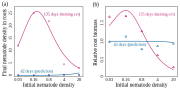
\includegraphics[width=\linewidth]{fig2.pdf} 
  \caption[Fit of the model to experimental data over one cropping
    season.]{Fit of the model to experimental data over one cropping
    season \citep{Ehwaeti1998}.  \textbf{(a)} Final density of
    nematodes in the roots and \textbf{(b)} relative biomass after 42
    (in blue) and 135 days (in magenta), as
    functions of the initial density of nematodes in the soil (log
    scale). Model outputs are shown as solid curves, circles and
    triangles represent experimental measurements.}
\label{fig2} 
\end{figure}

Parameters characterising virulent nematodes, \textit{i.e.}\ the fitness costs,  were selected from data on the \textit{Mi-1} resistant tomato  \citet{Castagnone-Sereno2007}. All parameters are summarised in \autoref{table1}.

\begin{table}[p]
  \small
  \caption{Model variables and parameters.}
  \label{table1}
  \begin{tabular}{@{}l@{ }l@{ }l@{ }l@{ }l@{ }l@{}}
    \hline
    Symbol & Description                      & Value(s) & & Unit &Ref.\\
    \hline
    $H^X$  & Density of healthy plant root    &          & & UR   & \\
    $P$    & Density of free living nematodes &          & & UN   & \\
    $E$    & Density of latently infected feeding sites& & & UR   &  \\
    $I$    & Density of infectious feeding sites &       & & UR   &  \\
    \hline
    $H_0$  & Initial root density & 6 &$(4.2,7.8)$ & UR & [1] \\
    $P_0$   & Initial nematode density in the soil & $0.8$ &$(0.03,20)$ & UN & [2] \\
    $p_v$ & Initial proportion of virulent nematodes & $10^{-3}$ &$(7\,10^{-4},1.3\,10^{-3})$ & -- & [3] \\
    $\beta$ & Infection rate & $1.11\,10^{-4}$ &$(7.78\,10^{-5},1.44\,10^{-4})$ & UR$^{-1}$ day$^{-1}$  & [*] \\
    $w_{\beta}$ & Fitness cost on infectiveness & $0.09$ &$(0.06, 0.12)$ & -- & [4] \\
    $\lambda$ & Transition rate from $E$ to $I$ & $0.06$ &$(0.042,0.078)$ & day$^{-1}$ & [4,5] \\
    $r$ & Nematode reproduction rate & $17$ &$(11.9, 22.1)$ & UN UR$^{-1}$ day$^{-1}$ & [4] \\
    $w_{r}$ & Fitness cost on reproduction & $0.31$ &$(0.22, 0.40)$ & -- & [4] \\
    $\delta$ & Fraction of  virulent offspring & $10^{-6}$ &$(7\, 10^{-7},1.3\,10^{-6})$ & -- & [3] \\
    $\alpha$ & Nematode mortality rate in roots & $0.125$ &$(0.0875, 0.1625)$ & day$^{-1}$  & [4,5] \\		
    $\eta$ & Nematode mortality rate in the soil & $0.04$ &$(0.028, 0.052)$ & day$^{-1}$ & [6] \\
    $\varphi$ & Between-season survival probability & $0.4$ &$(0.28, 0.52)$ & -- & [7] \\
    $\epsilon_y^X$ & Nematode infection success & \multicolumn{2}{@{ }l}{
                                                    \begin{tabular}[t]{@{}l@{}}
                                                      0 if $X=R$ and $y=a$\\[-6pt]
                                                      1 otherwise
                                                    \end{tabular}
    } & UR UN$^{-1}$  & \\		
    $\mu\,x$ & Plant root growth rate & $0.42$ &$(0.294, 0.546)$ &UR day$^{-1}$ & [1*]  \\
    $k$ & Nematode impact on root growth & $10.33$ &$(7.23,13.43)$ & -- & [*] \\ 
    $\tau$ &  Duration of a cropping season & $135$ & & days & [8] \\
    \hline
  \end{tabular}
  \par\medskip\footnotesize
  All parameters, except  $\epsilon_y^X$ and $\tau$, were varied for the sensitivity and robustness analyses: default value and $\pm 30\%$ variations  (indicated in brackets) were tested; larger variations were tested for $P_0$, in line with \citet{Ehwaeti1998}. \\
  \textbf{Units:} UR: number of feeding sites per gram of soil; UN: number of nematodes per gram of soil.  \\
  \textbf{Sources}: [1] \citet{Leskovar1990}; [2] \citet{Ehwaeti1998};
  [3] \citet{Ploeg1999}; [4] \citet{Castagnone-Sereno2007}; [5]
  \citet{Ekanayake1986}; [6] \citet{Tsai2008}; [7] Castagnone-Sereno, C.,
  unpublished data; [8] Djian-Caporalino, C., unpublished data; [8]
  Djian-Caporalino, C., unpublished data; [*] Estimated.
\end{table}

\subsection{Performance of resistance deployment strategies}
\label{sec:hrd}
We considered several resistance deployment strategies: the two
``pure'' resistant-only and susceptible-only strategies, consisting in
planting one crop type all the time; periodic rotation strategies,
alternating resistant and susceptible plants according to a repeated
pattern; and unconstrained strategies, \textit{i.e.}\ arbitrary
sequences of susceptible and resistant plants.

The performance of {each} strategy was quantified
with the ``healthy root density'' ($\overline{HRD}$), a proxy of
crop yield defined as the mean of the integral of healthy plant root
densities over the $n$ cropping seasons: 
\begin{equation}
  \overline{HRD}=\frac{1}{n} \sum_{i=1}^{n} \int_{i^{\text{th}}\text{ season}} H^{X}(t) dt
  \label{hrp}
\end{equation}
This quantity is similar to the healthy leaf area duration ($HAD$),
the integral of healthy green canopy area during a growing season,
used by many authors for airborne pathogens \citep{Waggoner1987,Gooding2000,vandenBosch2003,LoIacono2012,Elderfield2018,Papaix2018}.

The durability of resistance was then defined as the number of
consecutive seasons the resistant crop can be planted without losing
more than $1\%$ of crop yield ($\overline{HRD}$), compared to the
first year the resistance is used.  This definition is close to the
``usefulness time'' used in \citet{vandenBosch2008}, \textit{i.e.}\
the number of seasons until the yield drops under a preset
threshold. Such a metric helps assess the severity of the resistance
breaking problem at hand.

\subsection{Acceptable, efficient, and optimal strategies}

In order to quantify the benefit of each resistance deployment
strategy (or lack thereof), we computed its relative gain. It is
defined as the gain in healthy root density ($\overline{HRD}$) that
the strategy provides over the resistant-only strategy, normalised by
the gain that the resistant-only strategy provides over the
susceptible-only strategy.  This is illustrated in \autoref{fig3}.
For a given number of cropping seasons, \textit{i.e.}\ a given time
horizon, a positive relative gain indicates that the strategy
outperforms the resistant-only strategy, whereas a negative value
indicates that the resistant-only strategy is better. By definition,
the relative gain of the resistant-only strategy is equal to zero.
This metric is useful to determine whether, and how much, rotation
strategies are an improved way to deploy plant resistance. Moreover,
it allows comparisons across parameter values and epidemic situations
(see also \citet{Fabre2015}).

Based on this metric, we identified three types of strategies
(\autoref{fig3}). The optimal strategy is defined as the strategy that
maximizes the crop yield proxy $\overline{HRD}$~\eqref{hrp} and thus
the relative gain. Efficient strategies are defined as all strategies
that provide a relative gain at least $50\%$ as high as the optimal
strategy.  Last, acceptable strategies are all strategies with a
positive relative gain, \textit{i.e.}\ strategies that outperform
(even modestly) the resistant-only strategy.In what follows, the main
topic of interest will be to improve the efficacy of resistant-plant
based nematode control strategies. Therefore, we will essentially
concentrate on efficient and optimal deployment strategies.

In order to identify optimal periodic strategies, we computed all
periodic rotation strategies, beginning with resistant crops and
alternating $m$ and $p$ seasons of resistant and susceptible plants,
respectively. We denoted by $mR+pS$ these periodic strategies. As an
example, \autoref{fig3}a displays the healthy root density
($\overline{HRD}$) of all periodic rotation strategies over a
15-season time horizon. The optimal periodic strategy is $1R+5S$,
which corresponds to 1 season of resistant plants followed by 5
seasons of susceptible plants, and so on. A graphical representation
in \autoref{fig3}b--d displays the nematode and plant root dynamics
over time. We also identified unconstrained optimal strategies by
using a genetic algorithm implemented through the \textsc{genalg} R
package
(\href{https://CRAN.R-project.org/package=genalg}{https://CRAN.R-project.org/package=genalg}).
A chromosome in the genetic algorithm represented a full sequence of
susceptible ($S$, coded as 0) or resistant ($R$, coded as 1) plants
over the time horizon considered.  The population of chromosomes
(population size: 200) was initiated with random chromosomes. At each
generation, the best $20\%$ of chromosomes (according to our yield
proxy) were retained to form the next generation, with mutation
occurring at rate 0.01 (default parameter values of the package). The
algorithm was run for 50 generations, for each time
horizon. Convergence generally occurred in no more than 10
generations. The best chromosomes in the final generation were used to
determine the set of optimal unconstrained strategies.  We determined
optimal strategies for time horizons between 1 and 30 cropping
seasons. We also reported the corresponding ratios of resistant
plants, \textit{i.e.}\ the number of seasons with resistant plants
divided by the total number of seasons.

\begin{figure}[ht]
  \centering
   \includegraphics[width=\linewidth]{fig3.pdf} 
  \caption[Performance    of all periodic rotation strategies over a 15-season time horizon.]
  {\textbf{(a)} Performance ($\overline{HRD}$, colour scale)
    of all periodic rotation strategies, according to their number of
    seasons of resistant (in columns) and susceptible (in rows)
    plants, over a 15-season time horizon; performance of the
    susceptible-only, resistant-only and optimal strategies are
    indicated on the color scale.  The relative gain is defined as the
    gain in performance obtained by shifting from the resistant-only
    to another strategy, relative to the gain in performance obtained
    by shifting from the susceptible-only to the resistant-only
    strategy. The optimal periodic rotation strategy $1R+5S$ is
    identified by a black dot. Dotted$-$ and plain$-$line framed
    strategies represent acceptable periodic rotation strategies
    (relative gain $>0$) and efficient periodic rotation strategies
    (relative gain $>50\%$ of the optimal relative
    gain). \textbf{(b--d)} Graphical representation of two strategies:
    the resistant-only strategy (in blue) and the $1R+5S$
    periodic strategy (in gold), which is optimal over a
    15-season time horizon; shaded areas correspond to the inbetween
    seasons. Default parameter values were used (\autoref{table1}).  }
  \label{fig3}
\end{figure}

\subsection{Parameter exploration and epidemic scenarios}

To asses the impact of parameter values, we performed a global
sensitivity analysis \citep{Saltelli2008} on the healthy root density
$\overline{HRD}$~\eqref{hrp}, the yield proxy which quantifies the
performance of the resistance deployment strategies. We used the
multi-seasonal model~\eqref{sys1} and simulated the optimal periodic
rotation strategy over a 15-season time horizon. We varied all
parameter values by $\pm 30\%$ (default values given in
\autoref{table1}), except for the initial nematode density in the soil
$P_0$, for which larger variations were tested, in line with
\citet{Ehwaeti1998}. More details are available in Supporting
Information Methods~S3. The most influential parameters were found to
be the nematode reproduction rate $r$, the infection rate $\beta$, the
nematode mortality rate in the soil $\eta$ and the nematode mortality
rate in the root $\alpha$, four epidemiological parameters which
explained more than $80\%$ of the total $\overline{HRD}$ variability
(supporting information Fig.~S3). By varying these parameters around
their default value, we defined four epidemic scenarios, corresponding
to different levels of epidemic severity, from Low to Extreme
(\autoref{table2}).

\begin{table}[ht]
  \centering
  \caption{Definition of the four epidemic scenarios based on the four most influential  parameters: nematode reproduction rate ($r$), infection rate ($\beta$), nematode mortality in the soil ($\eta$) and in the roots ($\alpha$).}
  \label{table2}
  \begin{tabular}{lccccc}
    \hline
    Scenario & $\beta$ & $r$     & $\alpha$ & $\eta$  \\
    \hline
    Low      & $-30\%$ & $-30\%$ & $+30\%$  & $+30\%$ \\
    Medium   & --      & --      & --       &  --     \\
    High     & $+30\%$ & $+30\%$ & --       &  --     \\
    Extreme  & $+30\%$ & $+30\%$ & $-30\%$  & $-30\%$ \\
    \hline
  \end{tabular}
  \par\medskip\footnotesize
  Default parameter values (--) or default values $\pm 30\%$ were used (all values in \autoref{table1}).
\end{table}

Furthermore, we analysed with particular attention the influence of the genetic
parameters (fitness costs $w_{\beta},\,w_{r}$ and proportion of
virulent offspring $\delta$), possibly in combination with the
 epidemic scenarios, on the nature and  relative gain
of optimal rotation strategies. Specifically, we sought to determine
when optimal rotation strategies could outperform the usual
resistant-only strategy and to what extent crop yield could be
increased by using such rotation strategies.

\subsection{Robustness to parameter uncertainty}

Finally, we evaluated the robustness of our results to determine to
what extent optimal periodic strategies would remain effective if
biological parameters were not known with perfect precision. For the
medium, high and extreme epidemic scenarios defined in
\autoref{table2}, the optimal periodic strategy was computed over a
15-season time horizon and its performance was tested against
$\pm 10\%$, $20\%$ and $30\%$ variations of all parameters except the
initial nematode density in the soil $P_0$, for which larger
variations were tested (\autoref{table1}). In contrast with the
analysis focusing on the impact of the genetic parameters, the
periodic strategy was not computed afresh when the parameters
varied. For each epidemic scenario, we explored the parameter space
using a fractional factorial design containing 2187 parameter
combinations. The design was obtained using the \textsc{planor} R
package
(\href{https://CRAN.R-project.org/package=planor}{https://CRAN.R-project.org/package=planor}).


% ****************   SECTION RESULTS  ***************%

\section{Results}
\label{sec:Res} 

\subsection{Optimal and efficient deployment strategies} \label{sec:optimal_eff}

The performances (crop yield proxy $\overline{HRD}$) of
pure, optimal and efficient deployment strategies are shown
in \autoref{fig4}a, for different time horizons and the default
parameters. As expected, the resistant-only, efficient and
optimal strategies outperformed the susceptible-only strategy, since
the deployment of resistance prevents infection by avirulent
nematodes. However, for these strategies, {the crop yield proxy}
decreased with the time horizon. This is also expected, as the
deployment of resistance also causes virulent nematodes to appear and
take over the nematode population.

\begin{figure}[htp]
  \centering
  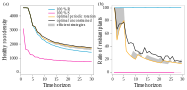
\includegraphics[width=\linewidth]{fig4.pdf} 
  \caption[(a) Performance and
    (b) ratio of resistant plants as functions of the time
    horizon, for different deployment strategie]{\textbf{(a)} Healthy root density ($\overline{HRD}$) and
    \textbf{(b)} ratio of resistant plants as functions of the time
    horizon, for different deployment strategies: susceptible-only
    (magenta), resistant-only (blue), efficient periodic rotations (grey
    area), optimal periodic rotation (gold) and optimal
    unconstrained (black). Different unconstrained optimal strategies
    (yielding the same $\overline{HRD}$) were identified, so the ratio
    of resistant plants is represented in panel (b) by its average
    value (the ratio range is represented in Supporting Information Fig.~S2). Default parameter values were used (\autoref{table1}).}
\label{fig4} 
\end{figure}

For up to five years of cultivation, the resistant-only strategy
performed as well as any optimal deployment strategy, but over longer
time horizons, it could be significantly outperformed. For instance,
over 15 cropping seasons, the {healthy root density} was around
$2044$~UR.day for optimal strategies, while it had dropped to
$1822$~UR.day for a pure resistant-only strategy (\autoref{fig4}a). By
definition, efficient periodic rotations performed better than the
resistant-only strategy and were worse than but close to the optimal
periodic rotation.  Interestingly, for all time horizons considered
(up to 30 years), the optimal periodic and the unconstrained
strategies had almost identical performances. This indicates that
periodic rotations are almost optimal in this system.

The deployment of a pure resistant-only strategy is thus reasonable
for at most five years in this cropping system. Beyond that, the
optimal strategy generally was to alternate one season of resistant
plants with a few seasons of susceptible plants, as shown for instance
in \autoref{fig3} for a 15-season time horizon. This optimal strategy
ensures that virulent nematodes remain sufficiently rare in the soil,
{sustaining} the efficiency of resistant plants, which severely reduce
the avirulent nematode population. Other periodic rotations
outperformed the resistant-only strategy. Yet, while there was
generally one single optimal periodic rotation strategy for a given
time horizon and parameter set, there were only a few acceptable and
even less efficient rotation strategies (\textit{e.g.}~10 acceptable
and 5 efficient strategies out of 105 periodic rotation strategies;
\autoref{fig3}a).


For a given time horizon, the average ratio of resistant plants
{characterizing} the unconstrained optimal strategy {was generally
  higher} than for the optimal periodic rotation strategy; for
acceptable and efficient periodic rotations, the ratio also tended to
be slightly higher than for the optimal periodic rotation
(\autoref{fig4}b).  For instance, over a 15-season time horizon, the
genetic algorithm identified 11 equivalent solutions and the ratio of
resistant plants deployed was on average $30\%$. For the optimal
periodic strategy, it was only $20\%$ and for acceptable and efficient
periodic rotation strategies, it ranged between $20\%$ and
$27\%$. Unconstrained optimal strategies identified by the genetic
algorithm were actually fairly similar to optimal periodic rotations
in terms of structure, except that more resistant plants were used in
the final seasons, explaining the higher ratio of resistant plants in
unconstrained strategies.

\subsection{Influence of fitness costs}

We computed the optimal periodic rotation strategies as functions of
the two fitness costs on infectiveness ($w_{\beta}$) and reproduction
($w_{r}$), to explore their effects on the two metrics defined above:
the relative gain brought about by optimal periodic rotations and the
resistance durability. Results are displayed in \autoref{fig5}a.

\begin{figure}[ht]
  \centering
   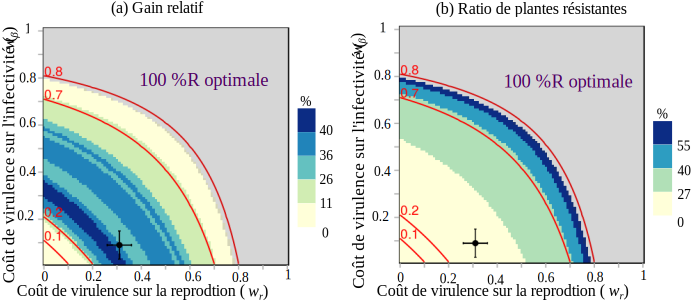
\includegraphics[width=\linewidth]{fig5.pdf} 
  \caption[(a) Relative gain and (b) ratio of
    resistant plants as functions of the two fitness costs, for
    optimal periodic strategies computed over a 15-season time
    horizon.]{\textbf{(a)} Relative gain and \textbf{(b)} ratio of
    resistant plants as functions of the two fitness costs, for
    optimal periodic strategies computed over a 15-season time
    horizon. The grey area corresponds to fitness costs for which the
    resistance was fully durable over the 15-season time horizon.
    Level curves in red represent different values of the effective
    fitness cost $w^*$ defined in \eqref{eff_w}. The black
    dot and the error bars indicate the default fitness costs and
    their standard deviations \citep{Castagnone-Sereno2007}.}
  \label{fig5}
\end{figure}

The area where resistance was durable for (at least) the entire
15-season time horizon is found in the upper right part of the figure.
This area corresponds to R-genes associated with very strong
fitness costs of one or the other kind ($w_{\beta}\geqslant 0.8$ or
$w_{r}\geqslant 0.8$). This means that rotation was unnecessary in such
conditions, at least for the time horizon considered. For lower
fitness costs, resistance was not durable and thus the use of optimal
periodic rotation strategies produced a better crop yield than the
resistant-only strategy (positive relative gain).

The relative gain was fairly high, except in two cases. On the one
hand, when resistance breaking entailed low fitness costs
($w_{\beta}$ or $w_{r}\leqslant 0.12$), the relative gain was almost
zero. This is not surprising since for such low fitness costs,
virulent nematodes cannot be prevented from overturning the nematode
population, even with rotation strategies, as they develop quite well
on both resistant and susceptible plants. Cropping resistant plants is
then useless and does not provide any increase in yield.  On the other
hand, R-genes associated with high fitness costs
($w_{\beta}$ or $w_{r}\geqslant 0.7$) provided a relative gain of less
than $10\%$. For such fitness costs, resistance durability was in fact
quite high (12 to 14 seasons). Therefore, the resistant-only strategy was quite efficient and
the additional yield provided by periodic rotations is minimal.

Significant relative gains are thus observed for R-genes inducing
medium fitness costs in virulent nematodes. Relative gains can in this
case reach values up to $50\%$. Interestingly, in the literature the
  fitness cost on reproduction $w_{r}$ is estimated between $0.26$ and
  $0.36$ and the fitness cost on infectiveness $w_{\beta}$ between $0.03$
  and $0.15$, for the susceptible Saint Pierre tomato cultivar \citep{Castagnone-Sereno2007}. For
such realistic fitness cost values, the expected relative gain that
could be realised by switching from a resistant-only strategy to an
optimal periodic rotation would be between $26\%$ and
  $43\%$  with a relative
gain equal to $28\%$  for the default values parameter values.

The ratio of resistant plants deployed in the optimal periodic
rotation strategies in order to achieve such relative gain values were
remarkably low, lying between $13\%$ and $27\%$
(\autoref{fig5}b). For the default parameter values, the
ratio of resistant plants was $20\%$. The ratio of
resistant plants used in the optimal rotation strategies increased
with the values of the fitness costs.

Interestingly, \autoref{fig5} shows that the fitness cost
distribution between infectiveness and reproduction is important for
crop yield. Indeed, even though the two fitness costs had perfectly
symmetrical effects, the level curves of both the relative gain and
the ratio of resistant plants were markedly concave. Therefore, a
balanced distribution of fitness costs (\textit{e.g.}\
$w_{\beta}=w_{r}=0.4$) could lead to a situation where resistance was
not durable, while an uneven distribution (\textit{e.g.}\ $w_{r}=0.8$,
$w_{\beta}=0$) could lead to a durable situation. The two fitness
costs thus did not act in an additive manner and interacted
negatively.  The derivation of the multiseason basic reproduction
number $R_{0}$ of virulent nematodes revealed that it depended only on
the product $(1-w_{\beta})(1-w_{r})$ (Supporting Information Methods~S1).  We hence defined an ``effective'' fitness cost as:
\begin{equation}
  w^{*}=1-(1-w_{\beta})(1-w_{r})=w_{\beta}+w_{r}-w_{\beta}w_{r},
  \label{eff_w}
\end{equation}
whose level curves perfectly reflected the level curves of the
relative gain and ratio of resistant plants
(\autoref{fig5}). The performance of resistance-based
strategies therefore appeared to be entirely determined by this
quantity.

In the following, we thus present results in terms of this effective
fitness cost $w^{*}$.

\subsection{Interplay between epidemic scenarios and  genetic parameters}

We studied the influence of the genetic parameters in interaction with
the epidemic scenarios on the relative gain and
durability. \autoref{fig6} shows the relative gain obtained for a
15-season time horizon as a function of the effective fitness cost
($w^*$), for different values of the fraction of virulent offspring
($\delta$) and the four epidemic scenarios. Parameter ranges ensuring resistance durability
over the 15-season time horizon were identified (grey areas).
$\delta$ had no effect on durability according to our
definition. Indeed, when only resistant plants were deployed,
avirulent nematodes could not reproduce. The resistance was durable as
the effective fitness cost $w^*$ {overshot} a given threshold, which
strongly increased with the severity of the epidemic scenario.  For
instance, for {low epidemic severity}, R-genes
associated with effective fitness costs between $0.30$ and $1$ were
durable (\autoref{fig6}a), while in the Extreme scenario, they
were durable only for fitness costs larger than $0.95$
(\autoref{fig6}d).

\begin{figure}[htp]
  \centering
   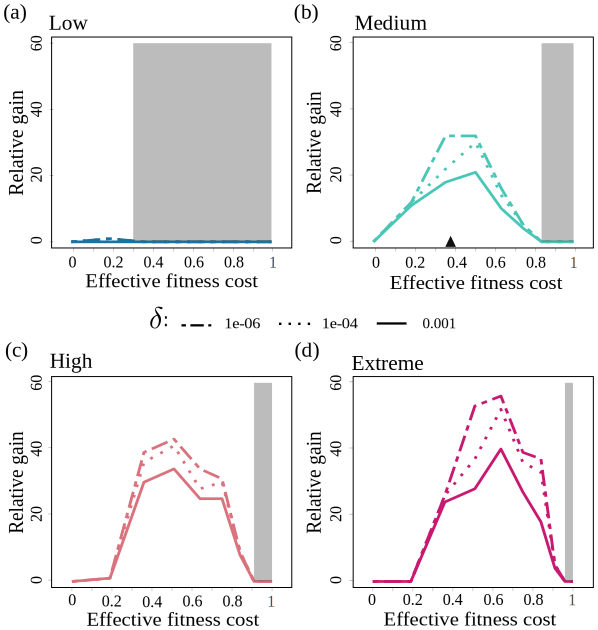
\includegraphics[width=.9\linewidth]{fig6.pdf} 
  \caption[Graphical representation of the relative gain for a
    15-season time horizon as function of epidemic scenarios]{Graphical representation of the relative gain for a
    15-season time horizon for the four epidemic scenarios
    (a-d) defined in \autoref{table2}, as a function of the effective
    fitness cost ($w^*$) and the fraction of virulent offspring
    ($\delta$). The default effective fitness cost $w^*=0.37$ is
    represented by the black triangle 
    \citep{Castagnone-Sereno2007}. Grey areas represent the values of
    $w^*$ for which the resistance was durable over the 15-season time
    horizon.}
  \label{fig6}
\end{figure}

The relative gain varied significantly according to the genetic
parameters and epidemic scenarios, except for the 
{Low epidemic scenario} where it remained close to zero
(\autoref{fig6}a). In this case, nematode infestation remained
very low so that the resistant-only strategy actually provided very
good control. The relative gain increased with {epidemic severity}
and decreased with the fraction of virulent offspring $\delta$. The
best gains were found for R-genes associated with medium to high
effective fitness costs (between $0.4$ to $0.65$). For example, an
extreme {severity} combined with a low fraction of
virulent offspring $\delta=10^{-6}$ and a fitness cost $w^*=0.65$
yielded a relative gain of up to $58\%$
(\autoref{fig6}d). Hence, {epidemic severity} tended to
increase the advantages of cultivar rotations over the resistant-only
strategy.

\subsection{Robustness of deployment strategies}

Finally, we evaluated the robustness of the optimal periodic rotation
strategies by testing their efficacy against variations in parameter
values.  \autoref{fig7} represents the relative gain when deploying
the optimal periodic strategy, computed over a 15-season time horizon
and for the default parameters corresponding to the three epidemic
scenarios, in the face of increasing levels of parameter variations.
Such variations can effectively render the computed rotation
strategies sub-optimal.

\begin{figure}[htp]
  \centering
   \includegraphics[width=.9\linewidth]{fig7.pdf} 
  \caption[Robustness of the relative gain to variations in model
    parameters]{Robustness of the relative gain to variations in model
    parameters, for three epidemic scenario (Medium, High, Extreme)
    and three levels of parameter variations ($\pm 10\%$, $20\%$,
    $30\%$, and variations in the initial nematode density as reported
    in \autoref{table1}). For each scenario, the optimal periodic
    strategy, computed for a 15-season time horizon and default
    parameters values (Tables~\ref{table1}--\ref{table2}) was
    applied. The relative gain of this strategy was computed for all
    parameter combinations within each level of parameter
    variations. In each case, the relative gains obtained for the
    default parameter values (black diamond) and for the different
    parameter combinations (2187 coloured dots) were plotted. Violin
    plots were drawn to help quantification, with horizontal bars
    indicating the median (thick line), first and third quartiles
    (thin lines). The percentages provided on the bottom line
    correspond to the fraction of parameter combinations which yield
    non positive relative gains, \textit{i.e.}\ for which the optimal
    strategy would not be acceptable (\autoref{fig3}).}
  \label{fig7} 
\end{figure}

In a large majority of cases, the relative gain remained positive,
although it declined, as expected, with the level of parameter
variations.  In the Medium epidemic scenario, most parameter
combinations decreased the relative gain below the $28\%$ gain
predicted for default parameter values (black diamond in
\autoref{fig7}). The median relative gain was between $8$ and $20\%$,
depending on the level of parameter variations. Note however
that some parameter combinations actually resulted in
higher-than-expected relative gains.  The situation was even more
favourable in the High and Extreme epidemic scenarios, for which the
decline in relative gain was less pronounced. In addition, a
significant fraction of parameter combinations caused an increase in
the relative performance of the optimal rotation strategy
(\autoref{fig7}).

Parameter combinations causing the rotation strategy to become
non-acceptable, \text{i.e.} for which the strategy failed to provide a
positive relative gain, were rare overall, especially for the most
severe epidemic scenarios. At most, these combinations represented
$18\%$ of all combinations (for $\pm 30\%$ variations in the Medium
epidemic scenario). The optimal strategy $1R+5S$, even in the face of
important parameter uncertainty, thus retained higher performance than
the resistant-only strategy in more than $82\%$ of the cases
tested. In that sense, the relative performance of the optimal
periodic strategy was globally very robust to parameter changes.


 

% *****************   SECTION DISCUSSION  ***************%

\section{Discussion}

\subsection{Crop rotation is an efficient strategy} \label{discussion:part1}

The present study was based on a new model of plant–nematode
interactions parameterized from the literature and fitted to
experimental data, so as to be representative of the tomato/root-knot
nematode system. As a key result, we found that alternating
susceptible and resistant plant cultivars in time can help limit the
proportion of virulent individuals in nematode populations and thereby
reduce crop loss substantially. According to our
simulations, relative gains as high as $40\%$ can be achieved,
compared to the baseline strategy of deploying only resistant plants,
over time horizons of 15 years or more.

The relative gain achievable with optimal crop rotations was found to
be greatest for high or extreme epidemic scenarios, \textit{i.e.}\  for
high {epidemic severities}. The latter result echoes previous findings
on the influence of epidemic intensity on resistance durability in the
context of spatial mixtures \citep{vandenBosch2003,Fabre2012}.  The
gain also increased, to a smaller extent, if the fraction of virulent
offspring in avirulent egg-clutches is smaller, and if the culture is
sustained over longer temporal horizons. Remarkably, the relative gain
obtained from virulence costs similar to those estimated for the
\textit{Mi-1} resistant gene is close to the maximum achievable gain
value (\autoref{fig5}a), suggesting that crop rotation is a
particularly promising strategy when deploying \textit{Mi-1}
cultivars.

We also found that periodic crop rotation strategies are almost as
effective as free (unconstrained) alternation strategies. This result
has considerable importance, since periodic rotation patterns are
in real-world applications much easier for crop growers to implement
than complicated unconstrained sequences. 

Few recent theoretical studies have considered the deployment of
different cultivars over time. One is
\citet{Rimbaud2018}, that compared four resistance deployment
strategies of major resistance genes: mosaics, mixtures, rotations and
pyramiding, to manage cereal rust fungi in agricultural landscapes
durably. They found cultivar rotation to be the most efficient in the
long-term, once every R-genes had been overcome. In a study of plant
virus epidemic control by mixing resistant and susceptible cultivars
in space and time, \citet{Fabre2015} identified that in more than
$20\%$ of the scenarios considered, optimal strategies involved
cultivar rotation at the landscape scale. Studies are even scarcer
regarding {root-knot nematodes}, for which the literature on cultivar rotation is
essentially experimental. For these low-dispersing soil-borne pests,
data support our modelling predictions in suggesting that rotations
are an effective way to reduce yield losses and to delay outbreaks
\citep{Tzortzakakis2000,Miller2006,McSorley2011}.  For instance,
\citet{Djian-Caporalino2014} experimentally compared the performance
of several strategies to control {root-knot nematodes} in vegetable cropping systems,
including rotations of two major R-genes in pepper cultivars, over
three years. They reported that cultivar rotation can improve
epidemic control and resistance durability. Another study by
\citet{Talavera2009} on {root-knot nematode} management compared the effects of four
crop rotations between resistant and susceptible tomato plants in a
three-year field experiment. Regarding crop yield and durability, this
study showed that the best strategy consisted in growing two resistant
cultivars, followed by one susceptible cultivar. This is strikingly
consistent with our modelling predictions, since we found that the
yield-maximising strategy, over a three-season temporal horizon, is
$2R + 1S$ (\autoref{fig4}b). Our modelling results further indicate
that the performance of crop rotations for {root-knot nematode} control would be even
more pronounced over longer time horizons.

\subsection{Crop rotation (usually) requires low ratios of resistant plants}  \label{sec:discussion-lowratio}

Interestingly, the optimal rotation strategies identified in this study
were characterised by relatively low ratios of resistant plants, as
soon as the temporal horizon exceeded seven cropping seasons (\autoref{fig5}b).
Since avirulent nematodes thrive on susceptible plants, low ratios
of resistant plants are expected to increase crop loss, especially
in the short-term. However, in the longer term, low ratios limit selection
for virulent variants, thus prolongating the efficacy of resistant
plants when those are deployed. For {root-knot nematodes}, it appears that the relatively
fast within-season epidemiological dynamics sets the optimal balance
between the two effects at a low ratio of resistant plants. Our results
are consistent with \citet{vandenBosch2003}, who showed that, in
many instances, low ratios allowed to make the most of resistance,
by reducing the selection pressure for virulent pathogens and promoting
resistance durability.

Interestingly, studies of spatial deployment strategies tend to report
higher optimal ratios of resistant plants. \citet{Fabre2012}, working
on plant resistance to viruses, demonstrated that optimal ratios were
frequently over $50\%$. For instance, for low fitness costs, the
ratio ranged between $50$ and $70\%$, depending on the epidemic
profile. Regarding phytopathogenic fungi, \citet{Papaix2014} also
found that high ratios combined with low levels of variety aggregation
provided optimal control of the fungi in agricultural landscapes.
Therefore, the selection pressure in favour of virulent variants seems
to be lower when mixing resistant and susceptible cultivars in space
compared to alternating them over time.

It should be remarked that low ratios of resistant plants are in total
contrast with the currently dominant agricultural practices, based on
the regular cropping of tomato cultivars bearing the same
\textit{Mi-1} resistance gene. Indeed, growing resistant tomatoes is
the best strategy over a single cropping season. However, be it in the
field or in experimental studies, such resistant-only strategies often
fail, and virulent {root-knot nematodes} overcoming resistance have
been observed in most tomato growing areas worldwide \citep{Seid2015}.
More specifically, experimental findings have shown that three
consecutive cropping seasons of the \textit{Mi-1} gene in tomatoes
were enough for {nematodes} to overcome the resistance
\citep{Eddaoudi1997,Verdejo-Lucas2009}.  These findings are consistent
with our results when fitness costs are not too severe, close to
available experimental estimates \citep{Castagnone-Sereno2007,
  Djian-Caporalino2011}.  The intense deployment of resistant
cultivars is thus bound to cause boom and bust cycles in this system
\citep{Brown2011}. During the boom, crop yield increases rapidly
thanks to the use of new resistant cultivar by growers and
farmers. Nevertheless, it is followed by a bust, characterised by the
rapid breakdown of the resistance by virulent variants and a drop in
crop yield. The switch to a new cultivar, carrying a fresh resistance
gene, then triggers a new cycle. To break this cycle and preserve the
efficiency of resistance genes, which are scarce and valuable
resources, cultivar rotations such as the ones proposed in this study
are a feasible and sustainable alternative. However, convincing
growers to switch from a short-term to a long-term perspective may be
an issue. It would require close interactions between scientists and
growers to co-design acceptable resistance deployment strategies.

\subsection{What makes a good resistance gene?}

We investigated the effects of varying three mechanistic parameters
characterizing how a resistance gene behaves with respect to
resistance breaking by {nematodes}: the fitness cost it imposes on the
infectivity of virulent nematodes ($w_{\beta}$), the fitness cost it
imposes on their reproduction ($w_{r}$), and the frequency of
virulence appearance in avirulent clutches ($\delta$). Obviously, one
would seek R-genes that, when overcome, would generate high values of
the first two parameters, and low values of the third, even
  though it may not necessarily be easy to evaluate.

Our results showed that the two fitness costs had interchangeable
effects in shaping the population dynamics of virulent
variants. However, the two costs interacted negatively, as the benefit
of increasing one fitness cost was reduced when the other fitness cost
is already high (\autoref{fig5}a). This original result
implies that, when evaluating the potential of resistance
genes to improve durability, breeders should seek and introgress
R-genes with maximal fitness cost on either one or the two components
of the nematode life-cycle (reproduction or infectivity), rather than
a balanced distribution of the two types of costs. To help address the
existence of two different types of fitness costs, a specificity of
our model, we derived a simple formula to synthesize the two fitness
costs into one effective fitness cost, according to which different
resistance genes can be ranked in terms of their
durability. Comparatively, the rate of production of virulent
nematodes $\delta$ had virtually no impact on the durability of
resistance genes.

Rotation strategies provided the largest relative
benefits over the resistant-only strategy for intermediate fitness
costs. Such measurements are not always easily accessible in the literature,
but this property seems to hold in a few other studies. For instance,
a reinvestigation of the simulation data on plant virus epidemics
obtained by \citet{Fabre2012} for high epidemic intensities showed
that the best relative gains were obtained for intermediate fitness
costs. Another study by \citet{Rousseau2019} showed that relative
additional gains, provided by combining quantitative and qualitative
resistances over qualitative resistances only, were most noticeable
for intermediate fitness costs. In both studies, the reasons for this
were similar to the present study: high fitness costs induced durable
resistance so that the yield could only be marginally increased, whereas
low costs induced poorly efficient resistance that did not benefit
from an optimal deployement. R-genes associated with intermediate
fitness costs are thus the ones that could benefit the most from improvements
in terms of deployment or cultivar genetic background.

\subsection{Optimal rotations in practice} \label{sec:discussion-OptRot-in-practice}
 
A major outcome of this work would be to recommend custom optimal
resistance deployment strategies to crop growers, depending on the
temporal horizon sought, but also on the epidemic context, the R-genes
to be deployed, and on the agricultural practices that determine model
parameter values. Indeed, even though optimal resistance deployment
has been proven to be efficient, quite few periodic rotation
strategies are actually ``acceptable'' and even less are ``efficient"
(\autoref{fig3}a). The pattern of the rotation, in particular the
ratio of resistant plants, is critical. In addition, soil infestation
and epidemiological or genetic parameters are particularly difficult
to estimate, and likely subject to considerable uncertainty. For
instance, \citet{Djian-Caporalino2011} found a large variability in
the fitness costs on reproduction. To address this issue, we simulated
the use of optimal periodic strategies, as computed for default
parameter values, and investigated how their performance responded to
parameter variations. We found that the relative gain was globally
robust to parameter changes. Thus, optimal periodic rotations can
outperform the resistant-only strategy in terms of crop yield even if
the relevant parameters are known imperfectly. Rotating susceptible
and resistant cultivars is not necessarily a good idea. However,
rotating wisely (optimally) can provide significant gains and is
robust to parameter uncertainties, which is a very desirable property
in practice.

There are still few studies that investigate the
robustness of resistance deployment strategies, or more generally
plant pathogen control methods. A similar analysis to parameter
misspecification was conducted by \citet{Hyatt-Twynam2017} to assess
the performance of optimal strategies to control the spread of citrus
canker in Florida, using one at a time epidemiological parameter
changes. In the context of fungicide resistance management,
\citet{Elderfield2018} found that mixtures always outperformed
alternations when parameters varied, but not the deployment
strategy. More such studies should arise to help bridge the gap
between theoretical resistance deployment strategies and their
implementation in the field.

Optimal strategies could feature high year-to-year variations in
yield, which may not be economically viable for farmers. Taking
advantage of the limited mobility of nematodes, this issue could be
adressed by implementing asynchronous crop rotation strategies in
different rows or plots, provided that contamination between those be
carefully avoided. The seasonal yield variations in each row would
average out, ensuring a more stable income for farmers while achieving
the performance of the optimal rotation strategy.

Although nematode resistance in general can be conferred by single
major genes or by combinations of genes or quantitative trait loci
(QTL), root-knot nematode resistance in solanaceous crops mainly
relies upon single major dominant genes
\citep{Barbary2015}. Currently, \textit{Mi-1} is the only resistance
gene used in tomato cultivars, which makes this study particularly
relevant for the tomato/root-knot nematode pathosystem. In pepper,
though, QTL have recently been identified \citep{Barbary2016} and
their efficiency was demonstrated in laboratory experiments
\citep{Barbary2014}. As such they could be a promising source of
resistance, alone or in combination with major R genes, which would
deserve further modelling investigations along the lines of the
present study. An ideal strategy would be to breed tomato varieties
with unbreakable resistance. In the absence of such a silver bullet, rotation of
varieties seems a viable alternative.

Provided sufficient parameter estimates are available, the model could
effortlessly be extended to simulate rotations of tomato with other
species (e.g.\ other Solanaceae or cucurbits), as is common in many
cropping systems. The present model could also readily be extended to
incorporate different R-genes and serve as a basis to evaluate more
complex resistance deployment strategies, involving rotations between
susceptible and several resistant cultivars or species, including
pyramided ones.


% ***************   ACKNOWLEDGEMENTS    ***************%

\section*{Acknowledgements}

This work was funded by INRAE and Région Sud PACA, France. It was certified by the Terralia-PASS competitiveness research cluster. The authors are grateful to the Inria Sophia Antipolis -- Méditerranée ``NEF'' computation cluster for providing resources and support.


\section*{Data availability statement}
The data that support the findings of this study are available from the corresponding author upon reasonable request.
